% Dependencias
\documentclass[a4paper,12pt]{report}

% Pacotes básicos
\usepackage[portuguese]{babel} % Idioma
\usepackage{graphicx} % Gráficos e imagens
\usepackage{amsmath} % Matemática avançada
\usepackage{geometry} % Margens e layout
\usepackage{setspace} % Espaçamento entre linhas
\usepackage{titlesec} % Personalização de títulos
\usepackage{tocloft} % Índice
\usepackage{longtable} % Tabelas longas
\usepackage{lipsum} % Texto fictício
\usepackage{enumitem} % Listas personalizáveis
\usepackage{fontspec} % Fontes personalizadas (necessário com XeLaTeX ou LuaLaTeX)
\usepackage{xcolor} % Cores
\usepackage[hidelinks]{hyperref} % Hiperlinks sem caixas
\usepackage{ragged2e} % Justificação de texto
\usepackage[natbibapa]{apacite} % Estilo APA para citações
\usepackage{url} % URLs
\usepackage{indentfirst} % Força a indentação do primeiro parágrafo

% Bibliografia
\bibliographystyle{apacite}

% Configuração de margens
\geometry{a4paper, top=2cm, bottom=2.5cm, left=2.5cm, right=2.5cm}

% Espaçamento entre linhas
\setstretch{1.5}

% Fontes
\setmainfont{Times New Roman}

% Configuração de títulos
% Configuração de títulos de capítulos alinhados à esquerda com tamanho 14pt
\titleformat{\chapter}[hang]
{\normalfont\bfseries\fontsize{14pt}{16pt}\selectfont} % Formatação do texto (14pt de tamanho, 16pt de espaçamento entre linhas)
{\thechapter.}{1em} % Número do capítulo seguido por um espaço de 1em
{\vspace{-1em}} % Reduz o espaço antes do título

% Configuração de subtítulos (sections) com tamanho 12pt
\titleformat{\section}[block]
{\normalfont\bfseries\fontsize{12pt}{14pt}\selectfont} % Formatação do texto (12pt de tamanho, 14pt de espaçamento entre linhas)
{\thesection}{1em}{}

% Configuração de títulos do Índice, Lista de Figuras e Lista de Tabelas
% Redefinir os títulos manualmente para o mesmo tamanho de fonte (14pt)
\addto\captionsportuguese{
	\renewcommand{\contentsname}{\fontsize{14pt}{16pt}\selectfont Índice}
	\renewcommand{\listfigurename}{\fontsize{14pt}{16pt}\selectfont Lista de Figuras}
	\renewcommand{\listtablename}{\fontsize{14pt}{16pt}\selectfont Lista de Tabelas}
}

% Ajuste de cabeçalhos
\usepackage{fancyhdr}
\fancypagestyle{conteudo}{
	\fancyhf{} % Limpa cabeçalhos e rodapés
	\fancyhead[R]{\small \nouppercase{\leftmark}} % Título do capítulo no canto superior direito
	\renewcommand{\headrulewidth}{0pt} % Remove a linha no cabeçalho
}

% Reduz o espaçamento entre linhas dos índices
\usepackage{etoolbox}
\patchcmd{\tableofcontents}{\@starttoc{toc}}{\@starttoc{toc}\setlength{\parskip}{-5pt}}{}{}
\patchcmd{\listoffigures}{\@starttoc{lof}}{\@starttoc{lof}\setlength{\parskip}{-5pt}}{}{}
\patchcmd{\listoftables}{\@starttoc{lot}}{\@starttoc{lot}\setlength{\parskip}{-5pt}}{}{}

% Configuração de cores
\definecolor{barraazul}{RGB}{0, 51, 153}

% Corrigir problemas de viúvas e órfãs
\clubpenalty=10000
\widowpenalty=10000
\sloppy


\begin{document}
	
	% Capa
	\begin{titlepage}
	\begin{flushleft}
		\begin{minipage}{\textwidth}
			\vspace{1cm} % Espaçamento antes da imagem
			
\includegraphics[width=0.5\textwidth]{iscte.png}
		\end{minipage}\\
	\end{flushleft}
	\noindent
	\textcolor{barraazul}{\rule{\textwidth}{1mm}} % Barra azul
	\\[0.5cm]
	{\Huge \textbf{\centering Desenvolvimento de modelos preditivos com base em RNN}}\\[1.5cm]
	\noindent
	\textbf{Luís Ricardo Silva Inácio}\\
	\textbf{Número de Aluno: 129074}\\[2cm]
	\textbf{Mestrado em Inteligência Artificial}\\[1.5cm]
	\textbf{Orientador: Tozé Brito, Phd}\\
	\textbf{Coorientador: Rui Brito, Phd}\\[3cm]
	\textbf{Outubro, 2024}
\end{titlepage}

	
	% Página em Branco
	% Página em Branco
\newpage
\thispagestyle{empty}
\mbox{}
\newpage
	
	% Contracapa
	\begin{titlepage}
	\begin{flushleft}
		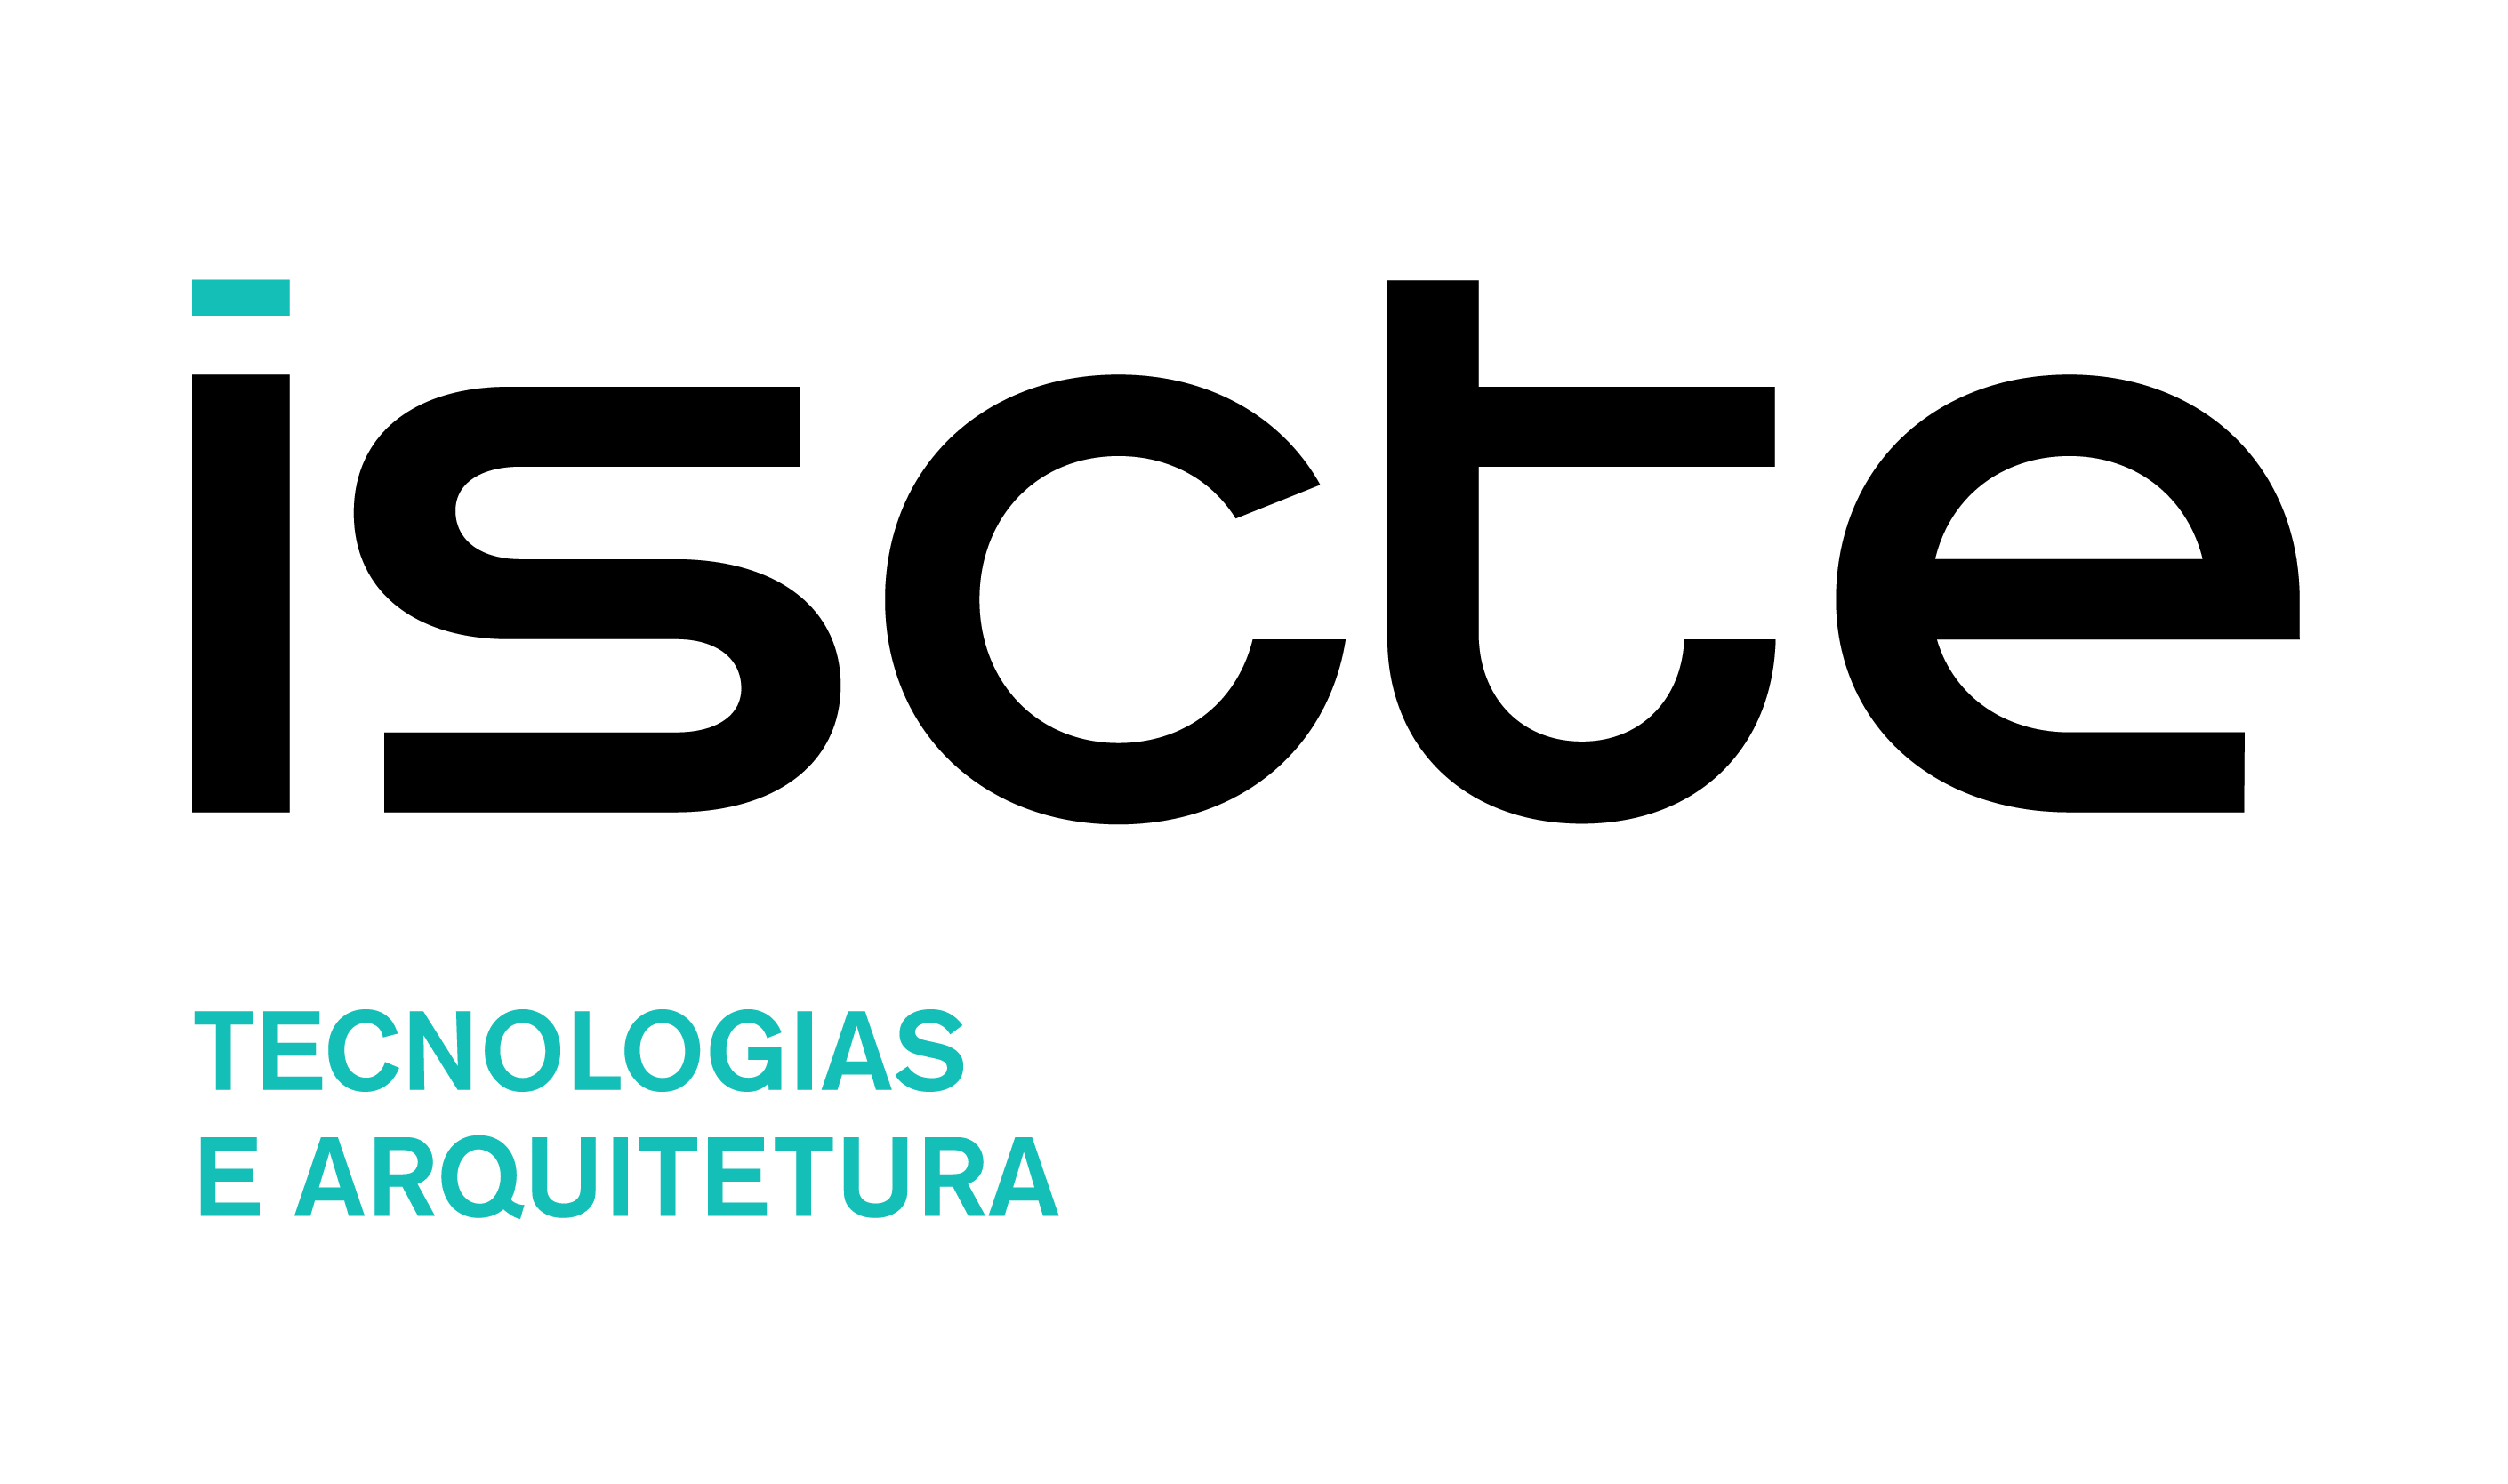
\includegraphics[width=0.5\textwidth]{ista.png}\\[1cm]
	\end{flushleft}
	\noindent
	\textcolor{barraazul}{\rule{\textwidth}{1mm}} % Barra azul
	\\[0.5cm]
	{\Large \textbf{\centering Departamento de Ciências e Tecnologias da Informação}}\\[1cm]
	{\Huge \textbf{\centering Desenvolvimento de modelos preditivos com base em RNN}}\\[1.5cm]
	\noindent
	\textbf{Luís Ricardo Silva Inácio}\\
	\textbf{Número de Aluno: 129074}\\[2cm]
	\textbf{Orientador: Tozé Brito, Phd}\\
	\textbf{Coorientador: Rui Brito, Phd}\\[3cm]
	\textbf{Outubro, 2024}
\end{titlepage}

	
	% Página de Copyright
	\newpage
\thispagestyle{empty}
\vspace*{1,5cm} % Adiciona uma margem superior fixa de 2 cm
\noindent % Evita indentação na primeira linha
{\footnotesize % Tamanho menor de texto (menor que \small)
	\textbf{Direitos de cópia ou Copyright} \\ % Título
	\textcopyright
	Copyright: Luís Ricardo Silva Inácio \\[-0.5cm] % Reduz o espaço após o autor
	\begin{flushleft} % Início do ambiente para alinhar à esquerda e justificar
		\renewcommand{\baselinestretch}{1}\selectfont % Define o espaçamento entre linhas
		\justify % Garante a justificação do texto
		O Iscte - Instituto Universitário de Lisboa tem o direito, perpétuo e sem limites geográficos, de arquivar e publicitar este trabalho através de exemplares impressos reproduzidos em papel ou de forma digital, ou por qualquer outro meio conhecido ou que venha a ser inventado, de o divulgar através de repositórios científicos e de admitir a sua cópia e distribuição com objetivos educacionais ou de investigação, não comerciais, desde que seja dado crédito ao autor e editor.
	\end{flushleft}
}
\newpage

	
	% Página de Agradecimentos
		% Página de Agradecimentos
\chapter*{Agradecimentos}
\addcontentsline{toc}{chapter}{Agradecimentos}
Gostaria de expressar a minha gratidão a todas as pessoas que me apoiaram durante a realização deste trabalho...
	
	% Resumo
	% Resumo
\newpage
\chapter*{Resumo}
\addcontentsline{toc}{chapter}{Resumo}
Texto do resumo em português. \\[1em]
\textbf{Palavras-chave:} palavra-chave1, palavra-chave2, palavra-chave3.
\newpage
	
	% Abstract
	\begin{abstract}
    This article provides a comprehensive review of the integration between OutSystems, Azure, and MongoDB, with a focus on facilitating large-scale applications. In the evolving landscape of software development, the collaboration between OutSystems' low-code platform, Microsoft's Azure cloud services, and the versatile MongoDB database offers a robust solution for addressing the complexities of extensive application deployments. The review encompasses key aspects such as architecture, scalability, and the seamless synergy achieved through this integration. Insights into practical implementations, challenges, and best practices are explored, offering valuable guidance for developers and enterprises seeking an optimal framework for large-scale application development and management.
\end{abstract}
	
	% Índices
	\tableofcontents
	\newpage
	\listoffigures
	\newpage
	\listoftables
	\newpage
	
	% Lista de Abreviaturas e Siglas
	% Lista de Abreviaturas e Siglas
\chapter*{Lista de Abreviaturas e Siglas}
\addcontentsline{toc}{chapter}{Lista de Abreviaturas e Siglas}
\begin{longtable}{p{3cm} p{10cm}}
	\textbf{Sigla} & \textbf{Descrição} \\
	\hline
	API & Application Programming Interface \\
	BI & Business Intelligence \\
	KPI & Key Performance Indicator \\
\end{longtable}

	
	% Começar numeração árabe
	\newpage
	\pagenumbering{arabic}
	
	% Capítulos
	\chapter{Introdução}
	A inteligência artificial tem evoluído significativamente nas últimas décadas, com avanços em redes neuronais profundas sendo especialmente notáveis. O livro seminal de \citet{goodfellow2016} destaca como o deep learning transformou o campo, permitindo o desenvolvimento de modelos complexos para problemas de visão computacional, linguagem natural e mais. Além disso, \citet{taylor2015} enfatiza que a simplicidade de certas abordagens pode ser essencial para iniciantes entenderem os fundamentos da aprendizagem automática. 
	
	Os desafios associados à implementação e otimização de redes neuronais foram explorados em várias pesquisas. Por exemplo, \citet{rao2019} argumenta que os principais desafios incluem o ajuste de hiperparâmetros e a escalabilidade dos modelos.
	
	\chapter{Revisão de Literatura}
	A literatura recente tem investigado estratégias para otimizar redes neuronais e melhorar a eficiência dos modelos. \citet{smith2021optimization} analisaram técnicas avançadas de otimização que têm um impacto direto no desempenho de redes neuronais em tarefas críticas. Da mesma forma, \citet{brown2020} exploraram o papel da aprendizagem automática na análise preditiva, destacando a importância do machine learning para setores como saúde e finanças.
	
	Um avanço importante foi a introdução de redes convolucionais para classificação de imagens por \citet{krizhevsky2012}, que revolucionou a área com a sua abordagem baseada no conjunto de dados ImageNet. Estudos subsequentes, como os apresentados em \citet{noauthor2021}, detalham os avanços em redes recorrentes, ampliando sua aplicabilidade em processamento de séries temporais e geração de texto.
	
	Contribuições teóricas também foram fundamentais. O livro \citet{mitpress2018} fornece uma base sólida sobre os princípios de aprendizagem profunda, enquanto \citet{wikipedia2024} oferece uma visão geral acessível das redes neuronais recorrentes.
	
	\chapter{Metodologia}
	A metodologia deste estudo foi baseada em abordagens sugeridas por \citet{smith2021optimization}, que enfatizam a utilização de técnicas otimizadas para treinar redes profundas. Além disso, os parâmetros do modelo foram ajustados com base nos princípios descritos por \citet{rao2019}, garantindo um equilíbrio entre desempenho e complexidade computacional.
	
	O framework experimental foi inspirado nas estratégias utilizadas em \citet{krizhevsky2012}, adaptando redes convolucionais para novos conjuntos de dados. Também foram incorporadas técnicas de análise preditiva baseadas nas metodologias descritas por \citet{brown2020}.
	
	\chapter{Resultados}
	Os resultados obtidos corroboram os achados de \citet{smith2021optimization}, demonstrando melhorias significativas na eficiência do modelo ao adotar técnicas avançadas de otimização. Adicionalmente, os modelos baseados em redes convolucionais apresentaram precisão semelhante às descritas por \citet{krizhevsky2012}, validando sua robustez em tarefas de classificação de imagens.
	
	Curiosamente, as limitações de redes recorrentes, como discutido por \citet{noauthor2021}, foram observadas em tarefas de processamento sequencial, reforçando a necessidade de arquiteturas híbridas para superar esses desafios.
	
	\chapter{Conclusão}
	Com base nas evidências apresentadas, pode-se concluir que a adoção de técnicas modernas de otimização e arquiteturas avançadas de redes neuronais desempenha um papel crucial no avanço da inteligência artificial. Conforme discutido em \citet{goodfellow2016}, o futuro do deep learning depende da contínua integração de métodos teóricos e práticos.
	
	Além disso, as contribuições de \citet{rao2019} e \citet{brown2020} destacam que uma abordagem multidisciplinar é essencial para enfrentar os desafios associados à escalabilidade e aplicação prática dos modelos. Este trabalho, portanto, reforça a importância da pesquisa colaborativa e interdisciplinar no progresso da inteligência artificial.
	
	% Referências Bibliográficas
	\addcontentsline{toc}{chapter}{Referências Bibliográficas}
	\bibliography{referencias}
	
	% Apêndices
	\appendix
	\chapter{Anexo A}
	Texto fictício para apêndice.
	\lipsum[10]
	
\end{document}
